\section{\texorpdfstring{AutoLibra 
\includegraphics[height=1em]{figs/scale.png}}{AutoLibra}}

To address the limitations of existing evaluation paradigms, AutoLibra \protect
\includegraphics[height=1em]{figs/scale.png} is designed to
meet the following desiderata: (1) \emph{data-driven}: This ensures that metrics are grounded
in real agent behavior and human opinions,  (2) \emph{self-validating}: Allows choosing minimal set of metrics that cover unseen human feedback with sufficient abstraction to be useful across different tasks, and (3) \emph{generalizable}: Applicable to various agent environments, independent of domain-specific design.

Based on feedback data collected from humans (\S\ref{sec:collecting-human-feedback}), AutoLibra achieves these desiderata through a closed-loop pipeline
consisting of two processes: \textbf{Induction Process} that converts agent behaviors and corresponding feedback into metrics, (\S\ref{sec:induction_process}) and \textbf{Evaluation Process} that predicts ratings and quality of new agent behaviors on the induced metrics (\S\ref{sec:evaluation_process}). 


\subsection{Collecting human feedback}
\label{sec:collecting-human-feedback}
In this paper, we use human feedback from two groups: (1) End-users -- for agents that interact directly with humans, we use the feedback from the users who interact and converse with the agents. CoGym \citep{shao2024collaborative}
is the environment that belongs to this category, and we use the user comments collected in their study, resulting
in 197 trajectories with feedback. (2) Experts -- for agents that
do not directly interact with humans, we use the feedback from human annotators (five authors in this paper) who observe agent trajectories. All other environments belong to this category, these being Sotopia \citep{zhousotopia}, WebArena \citep{zhouwebarena}, WebVoyager \citep{he2024webvoyager}, Baba-is-ai \citep{cloos2024babaaibreakrules}, and MiniHack \citep{samvelyan2021minihackplanetsandboxopenended}. For each trajectory, we collect only one element of feedback; feedback is given based on the complete agent trajectories.\footnote{While in theory we can leverage feedback on specific steps to achieve better feedback grounding and multiple feedback for single trajectory, we leave it as future work.}

\begin{wrapfigure}[17]{r}{0.4\linewidth}
  \vspace{-15pt}
  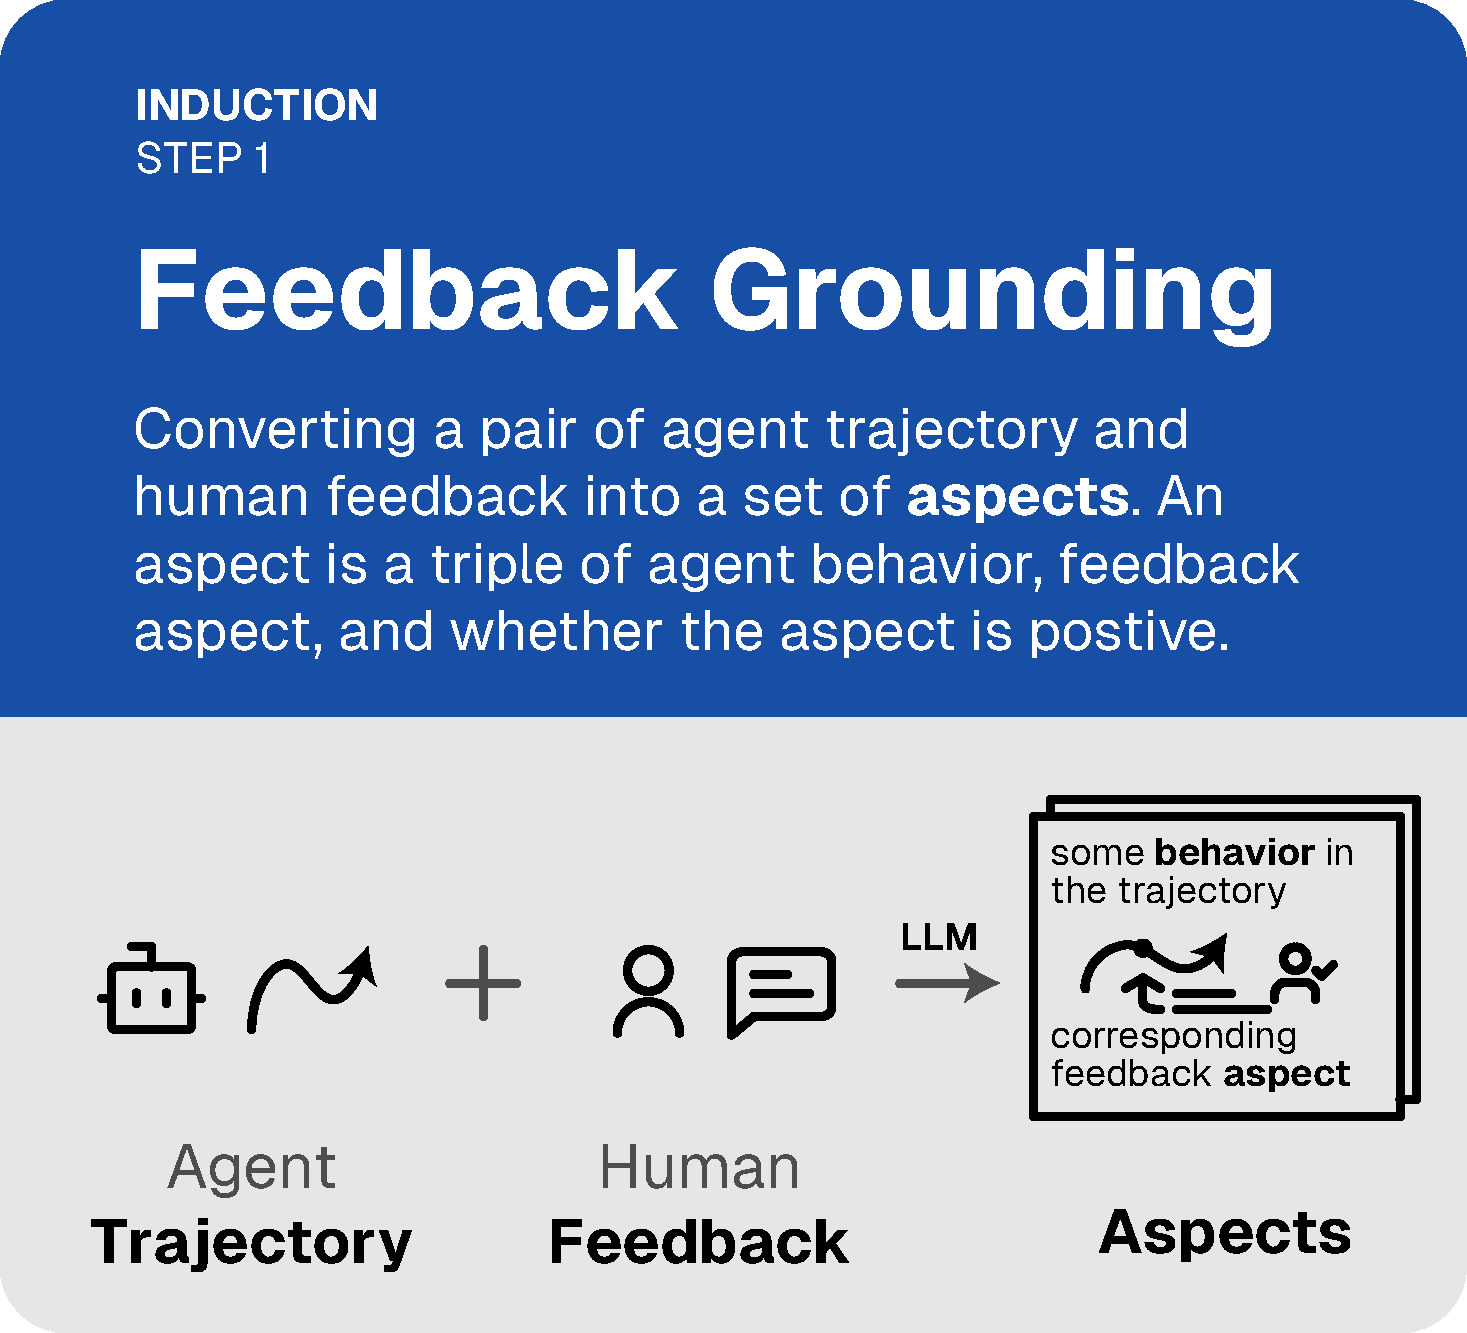
\includegraphics[width=\linewidth]{figs/autolibra_step_1.pdf}
  \vspace{-10pt}
  \caption{Feedback Grounding}
  \label{fig:feedback_grounding}
\end{wrapfigure}
Annotators are instructed to explicitly indicate the aspects of agent behavior that they classify as good or bad,
and to avoid general comments such as \textsf{"The agent is good at solving the task"}.
The annotators can also choose from a TTY (TeleTYpewriter) or a web interface; in both cases the annotator is provided with the agent's task
and then view the agent's observation and actions step by step, in text form. \footnote{While viewing screenshots is standard for web navigation tasks, we keep the observation format consistent across agents and humans to encourage more grounded feedback.}
For multi-agent tasks, we annotate each agent's trajectory in a given interaction separately. For Sotopia \citep{zhousotopia}, WebArena \citep{zhouwebarena},
and WebVoyager \citep{he2024webvoyager}, we annotate 100 trajectories of agents based on GPT-4 \citep{achiam2023gpt} with feedback for each dataset. For experiments in \S\ref{sec:ladder} we annotate 18 trajectories for each dataset in each
iteration. The annotation process is fast: Human annotators spend less than 5 minutes to provide feedback for each trajectory; \S\ref{sec:lens}, we further randomly hold out 20\% of the trajectories for validation.

% \begin{figure}
%     \centering
%     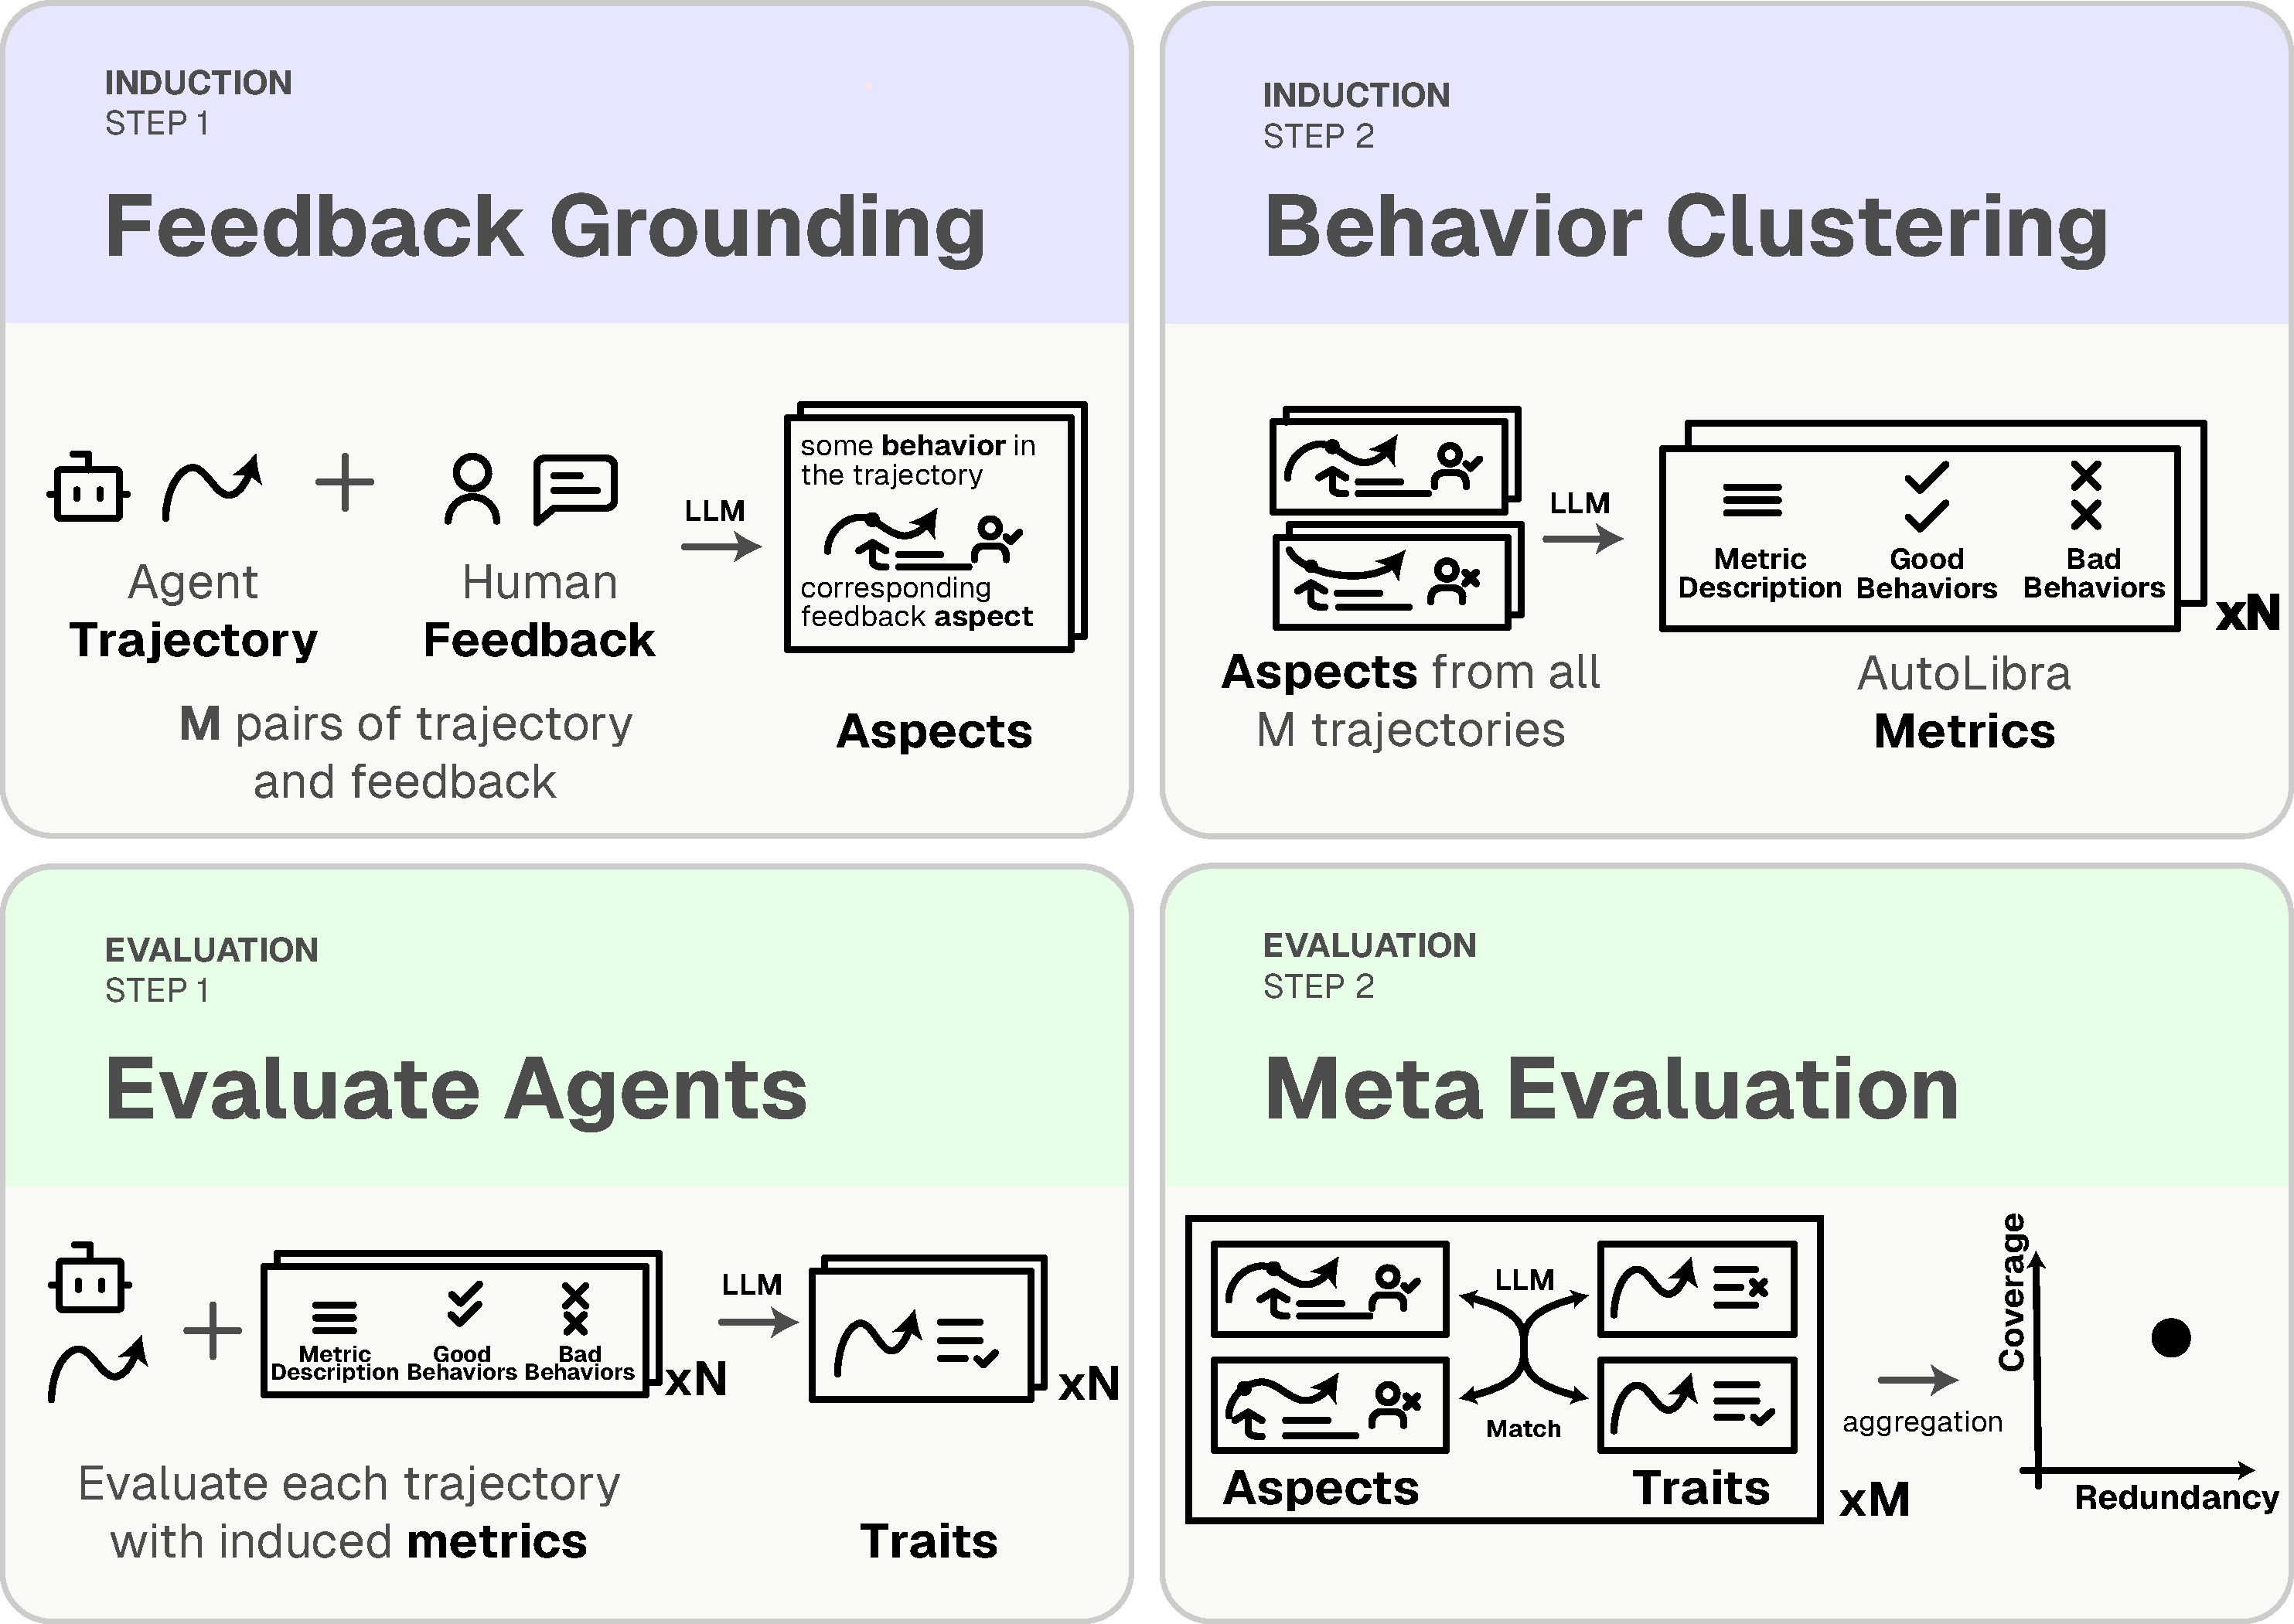
\includegraphics[width=\linewidth]{figs/autolibra_pipeline_v2.pdf}
%     \caption{Caption}
% Caption    \label{fig:enter-label}
% \end{figure}


\subsection{Induction Process: agent trajectories and human feedback $\rightarrow$ evaluation metrics}
\label{sec:induction_process}

\paragraph{Feedback Grounding}
The feedback of human annotators can contain multiple aspects; e.g. \textsf{``AI agent was pretty good
at giving me a consistent itinerary and vacation plan, although it froze on the last couple of minutes.''},
%\diyi{are all feedback from cogym? the current writeup is confusing and easily get readers to think about the feedback is from cogym only. if not, we need to add a few sentences saying how feedback is achieved, and how easy it is for humans to provide such feedback. otherwise, if this is something taking a lot of time, why do we want to use it?} 
collected from human annotators in CoGym \citep{shao2024collaborative}, contains a positive aspect
about the agent's ability to generate a consistent itinerary, and a negative aspect about the agent freezing
at the end. Here we define an \emph{aspect} as a triple $(\texttt{behavior}, \texttt{feedback}, \texttt{sign})$.
In the positive aspect of the previous example, the \texttt{behavior} is the agent's actions to create
a 20-day itinerary for the Maldives, the \texttt{feedback} is that the created itinerary is consistent and the \texttt{sign} is positive. This grounding procedure is similar to the coding procedure in thematic analysis by humans.



Illustrated in Fig. \ref{fig:feedback_grounding}, in this step, we feed the trajectory and the feedback into the LLM (we use GPT-4o \citep{openai2024gpt4ocard} 
as it yields good results in our experiments) and prompt the LLM with the following instructions:
(1) break down the feedback into bullet points; (2) for each bullet point, find the corresponding
part of the trajectory to which the feedback refers. Finally, we use constrained decoding to force GPT-4o
to output the aspects in the previous format. In our experiments, we find that on most datasets, for each
trajectory, the LLM can generate one to five aspects, with a mean of one to two aspects.


\paragraph{Behavior Clustering}
\begin{wrapfigure}[16]{l}{0.4\linewidth}
  \vspace{-15pt}
  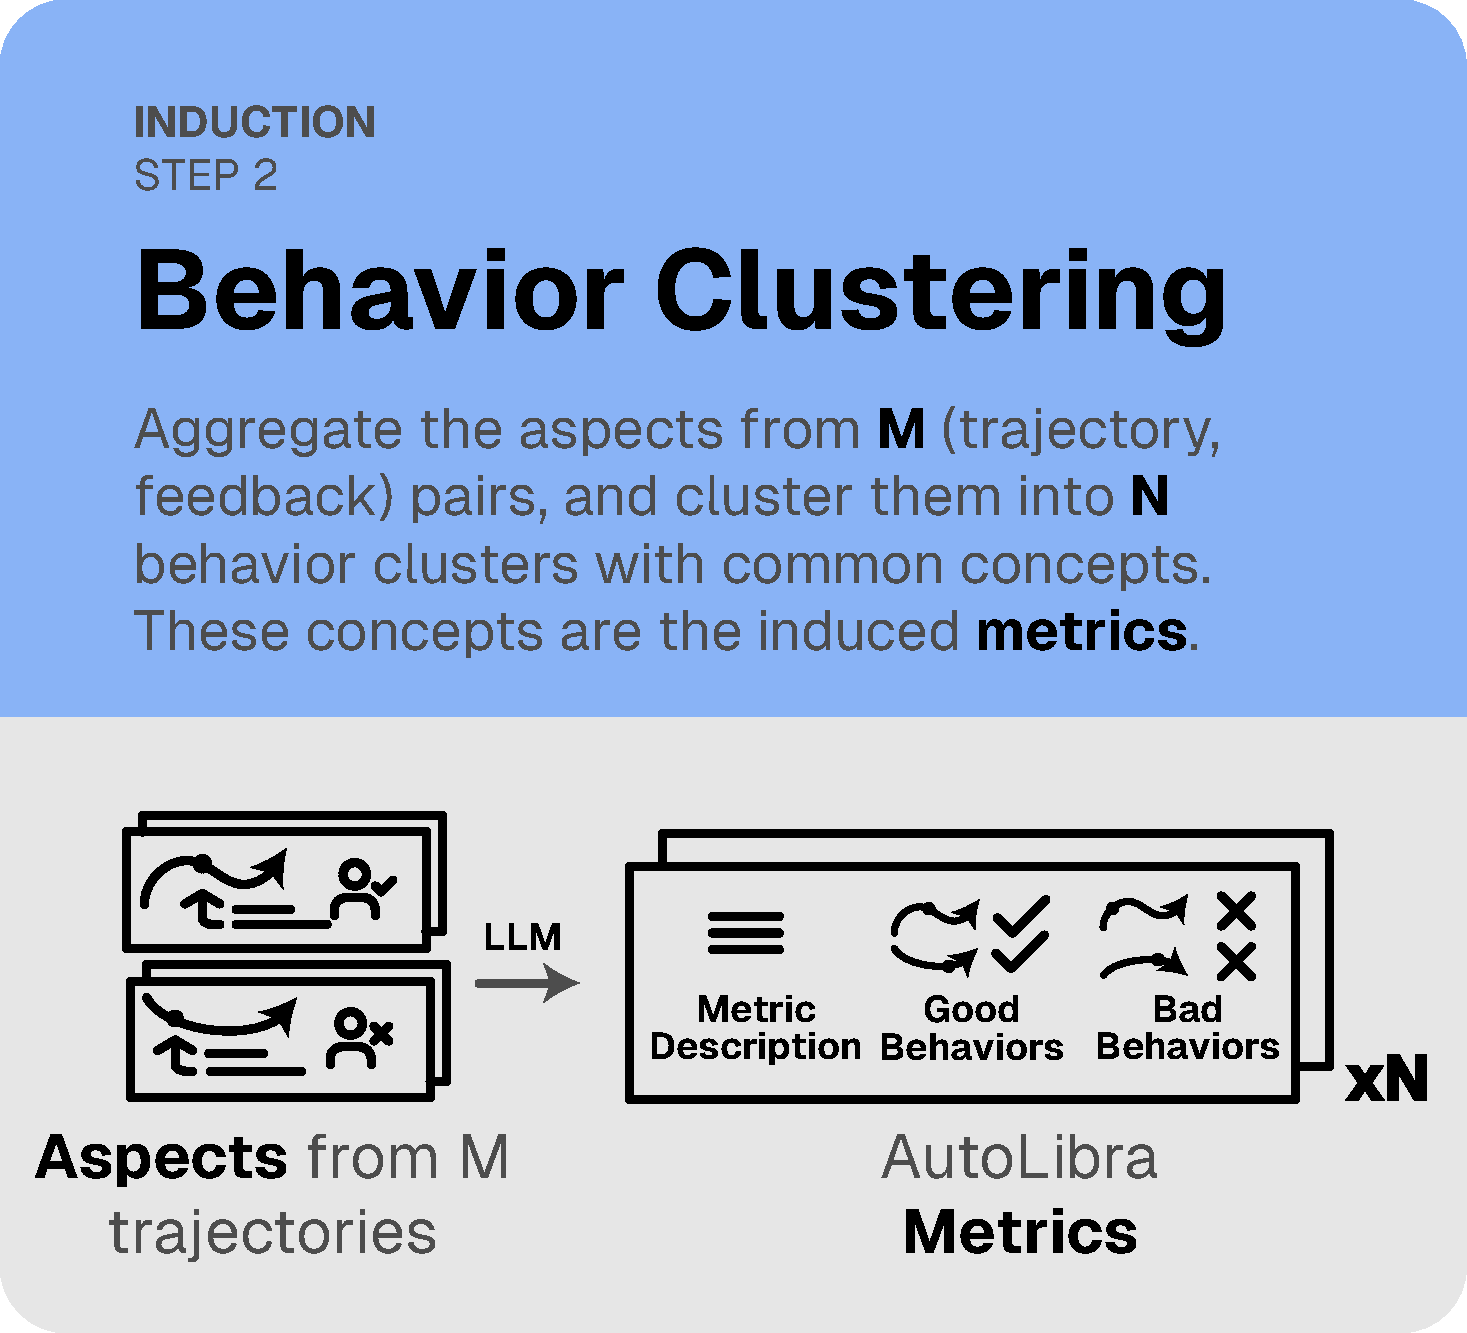
\includegraphics[width=\linewidth]{figs/autolibra_step_2.pdf}
  \vspace{-10pt}
  \caption{Behavior Clustering}
  \label{fig:behavior_clustering}
\end{wrapfigure}
The second step of the extraction process is to group the aspects into $N$ metrics.
To illustrate this step, we consider another example in the same dataset
\textsf{``The AI responds quickly to write and run the Python script``} where
the \texttt{behavior} is the agent's action to quickly write and run a Python script, the \texttt{feedback}
is that the agent responds quickly, and the \texttt{sign} is positive. Although this aspect is a positive aspect,
it reflects the same dimension of the agent's behavior as the previous negative aspect, with an opposite value.
Each \emph{metric} is a cluster of aspects, with a definition summarizing the criteria of positive behaviors, a list of positive behavior examples, and a list of negative behavior examples. This clustering procedure
is similar to the theme induction step in thematic analysis.

However, clustering similar agent behaviors together is challenging for statistical clustering methods.\footnote{
    In preliminary experiments, we tried to use K-means clustering on the aspect vectors generated by \texttt{text-embedding-3-large},
    but the clusters are mostly based on tasks and not on the behaviors.
}
Inspired by LLM-based semantic clustering and concept induction methods \citet{viswanathan2024large,lam2024concept}, we prompt an LLM (o3-mini high\footnote{https://openai.com/index/openai-o3-mini/}, as it produces the most accurate coverage and redundancy scores as evaluated later) 
to cluster the aspects into metrics. 
As illustrated in Fig. \ref{fig:behavior_clustering},
we gather all the aspects of $M$ trajectories
and cluster into $N$ metrics, where $N$ is a parameter set through the optimization process (\S\ref{sec:metric-optimization}).
We provide the LLM with the following instructions:
\emph{The granularity of the grouping should be minimal; only very similar behaviors are grouped together; but don't limit to one particular website or one particular character}, which empirically
makes the metrics more concrete but still applicable across different tasks.


\subsection{Evaluation Process: evaluating agents and the quality of the induced metrics}
\label{sec:evaluation_process}

\paragraph{Evaluating agents with induced metrics}
LLM-as-a-Judge \citep{zheng2023judging},
or more broadly, model-based evaluation
\citep{zhang2019bertscore,celikyilmaz2021evaluationtextgenerationsurvey}
is a method to use machine learning models to evaluate the output of other machine learning models.
The success of LLM-as-a-Judge depends on the gap between the difficulty of evaluation or verification and
that of generation and action. 
In agentic tasks, this gap is often large, as the policy model must perform multiple steps in decision-making, while the evaluation model must only
classify the trajectories, which make LLM-as-a-Judge widely used \citep{zhouwebarena,he2024webvoyager,zhousotopia}.
In AutoLibra, we employ LLM-as-a-Judge to
evaluate the agent trajectories configured with the induced metrics. However, LLM-as-a-Judge
can be replaced by any other evaluation methods implementing the induced metrics;
\emph{e.g.} an \texttt{interact-valid-element} metric
could be evaluated by a rule-based evaluator that checks if the agent
interacts with valid elements on the webpage. We note that AutoLibra could be used with other evaluation methods, such as
programmatic evaluation \citep{maeureka}; we leave generating programs for the induced metrics for future work.

\begin{wrapfigure}[16]{r}{0.4\linewidth}
  \vspace{-15pt}
  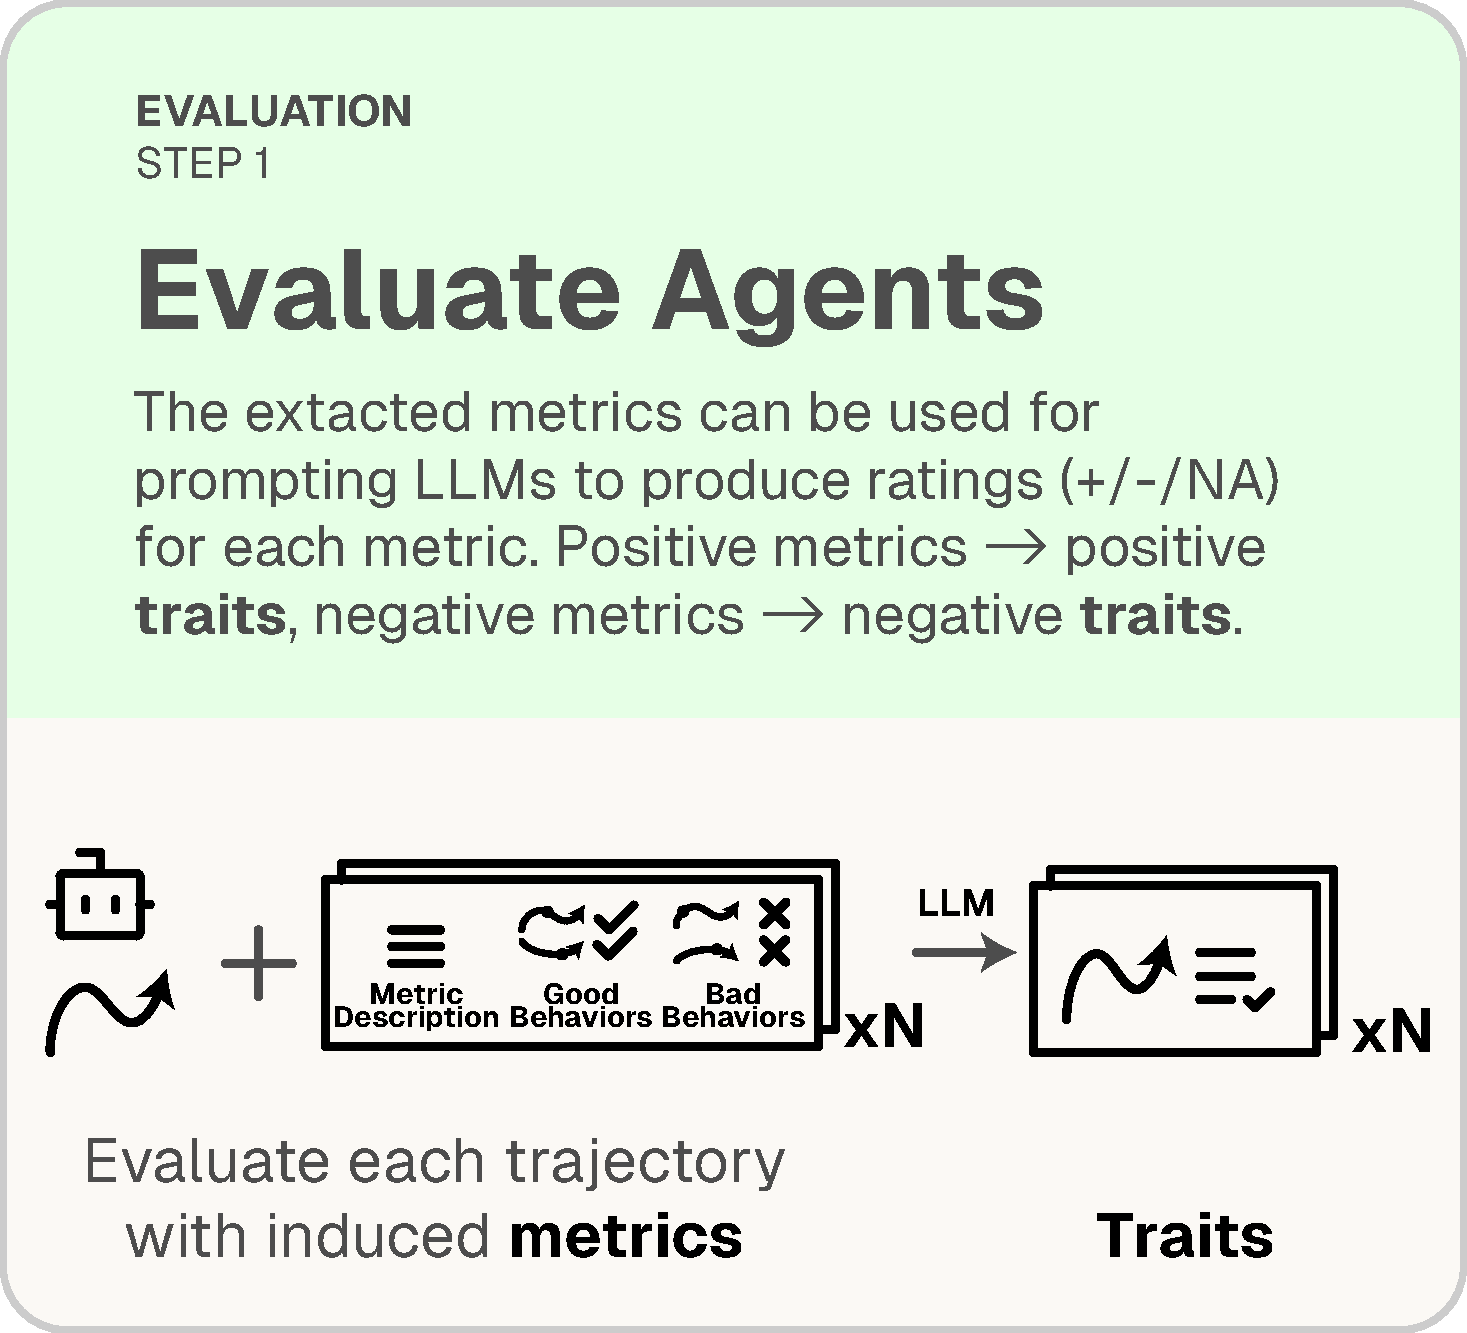
\includegraphics[width=\linewidth]{figs/autolibra_step_3.pdf}
  \vspace{-10pt}
  \caption{\small Evaluating agents with induced metrics}
  \label{fig:llm_as_a_judge}
\end{wrapfigure}
As illustrated in Fig. \ref{fig:llm_as_a_judge}, taking the induced metrics as input, an LLM (we use o3-mini medium,
as it provides similar results in this step to o3-mini high) is prompted to rate the agent trajectories to \{+ 1, -1, N / A\} for each metric. For an agent trajectory, the metrics labeled +1 are
the positive \emph{traits}, and the ones labeled -1 are the negative \emph{traits}. When we calculate the scores of
the metrics, we use the ratio of agent trajectories rated as positive
to the ones that are rated as positive or negative, ignoring those rated as N/A,
since not all metrics are applicable to all trajectories
(some metrics like \texttt{valid-search-terms} are only applicable when the task
involves searching). 


\paragraph{Meta evaluation}
The last component of the loop is the meta-evaluation, i.e. evaluating the evaluation metrics induced by AutoLibra.
This step matches the traits detected by the LLM-as-a-Judge with aspects
grounded from the human feedback. The goal is to verify whether (1) the induced metrics cover the behaviors the human annotators care about, and (2) LLM-as-a-Judge can produce
accurate evaluation results based on the induced metrics. In the previous example,
if the \texttt{respond-promptly} is extracted as a metric, and the LLM-as-a-Judge
has the same opinion as the human annotators, then this aspect is considered as successfully covered.
If either a similar metric was not extracted, or the LLM-as-a-Judge assigns a different score,
then this aspect is considered as not covered.

\begin{wrapfigure}[15]{l}{0.4\textwidth}
  \vspace{-15pt}
  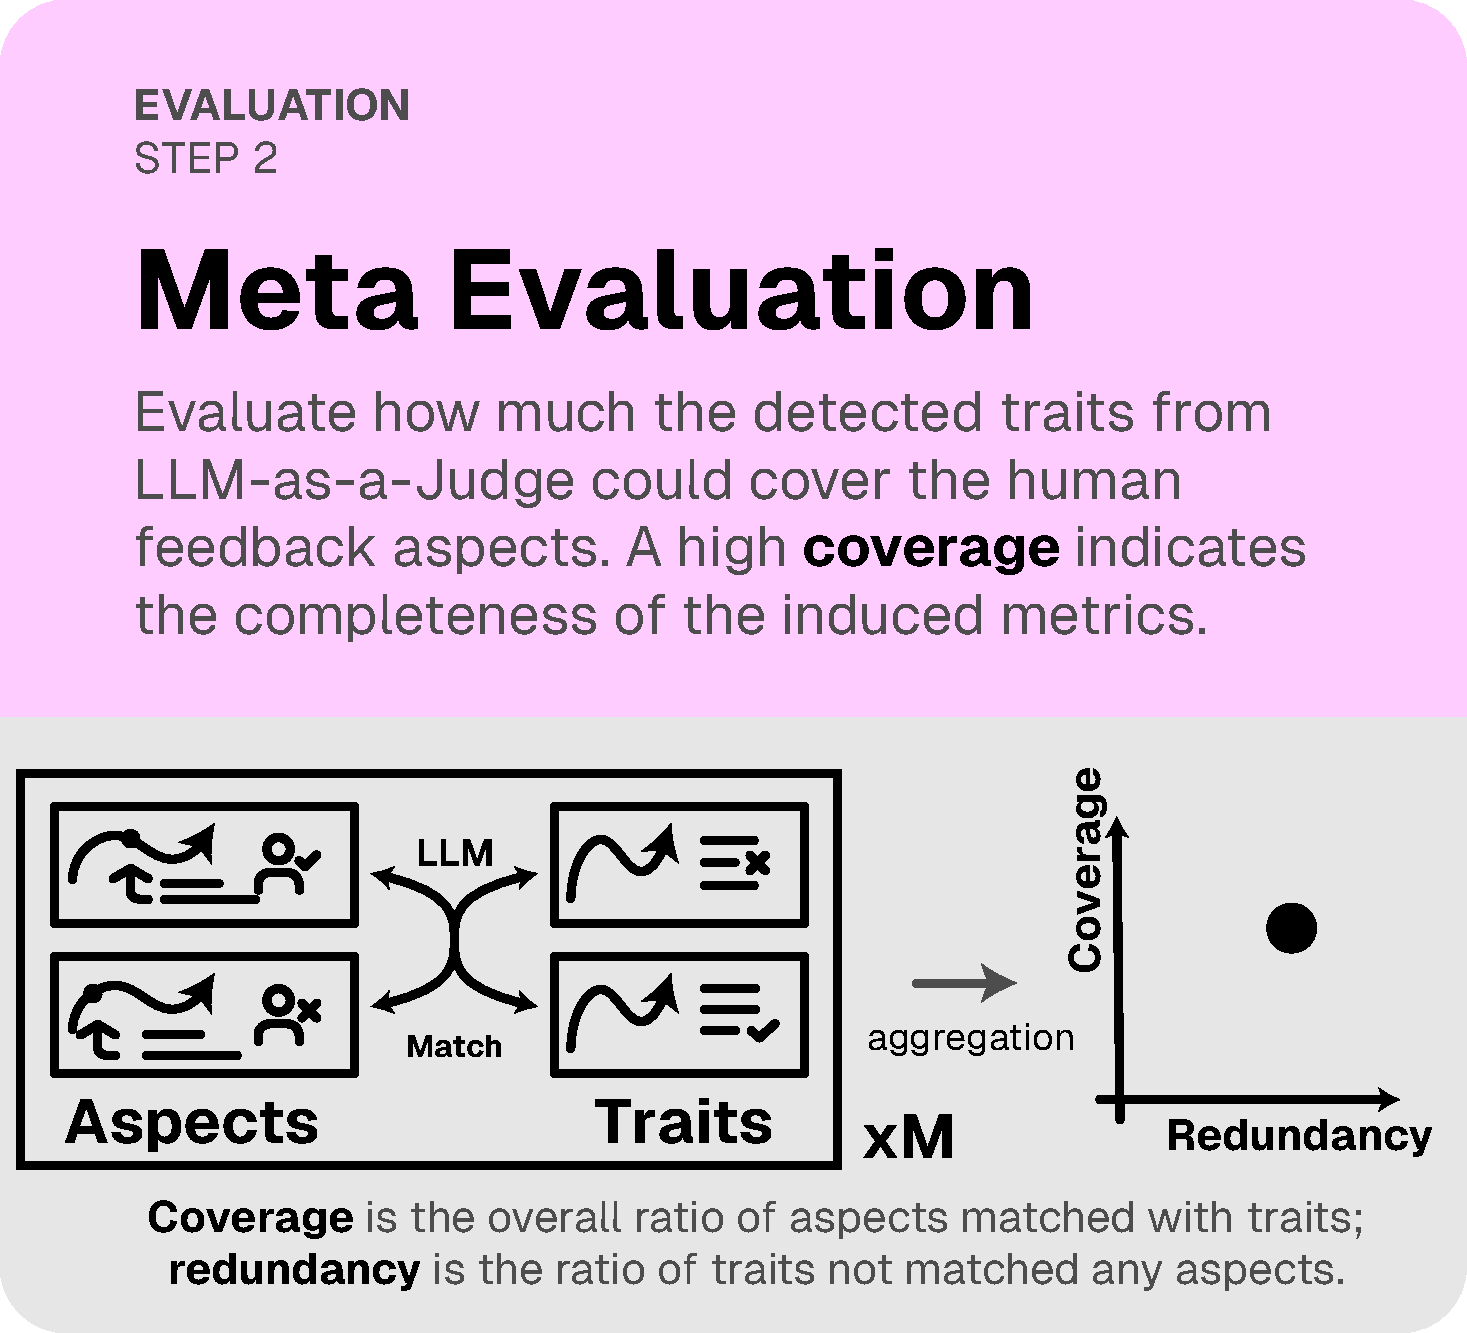
\includegraphics[width=\linewidth]{figs/autolibra_step_4.pdf}
  \vspace{-10pt}
  \caption{\small Meta evaluation}
  \label{fig:meta_evaluation}
\end{wrapfigure}
Illustrated in Fig. \ref{fig:meta_evaluation}, to perform this step, for each trajectory-feedback pair, we classify the aspects into positive and negative aspects, classify
traits into positive and negative traits, then attempt to match the positive aspects with positive traits
and the negative aspects with negative traits. 
We prompt an LLM (we use GPT-4o \citep{openai2024gpt4ocard},
as it gives good results in our experiments) with a list of aspects and another list of traits
and ask the LLM to find the best matching trait for each aspect or decide that there is no matching trait.
The \emph{coverage} of the whole dataset is calculated as the  proportion of aspects of all instances that have a matching trait,
and the \emph{redundancy} is calculated as the proportion of traits of all instances that have not been matched to any aspect.

\section{Optimizing and validating AutoLibra \protect
\includegraphics[height=1em]{figs/scale.png}}
AutoLibra is designed to be self-validating through the evaluation process, which allows us to search the optimal set of metrics that cover the human opinion the best (\S\ref{sec:metric-optimization}). 
This optimization process can also be applied iteratively throughout the agent improvement process: As the agent is optimized, new metrics can be added to existing metrics (\S\ref{sec:iterative-induction}), which is similar to how unit tests are kept throughout software development to prevent new features from interfere with existing features. 
In the last part of this section, we study the alignment between each step of AutoLibra and human judgment. 


\subsection{Metric Optimization}
\label{sec:metric-optimization}

\begin{figure}[!t]
    \centering
    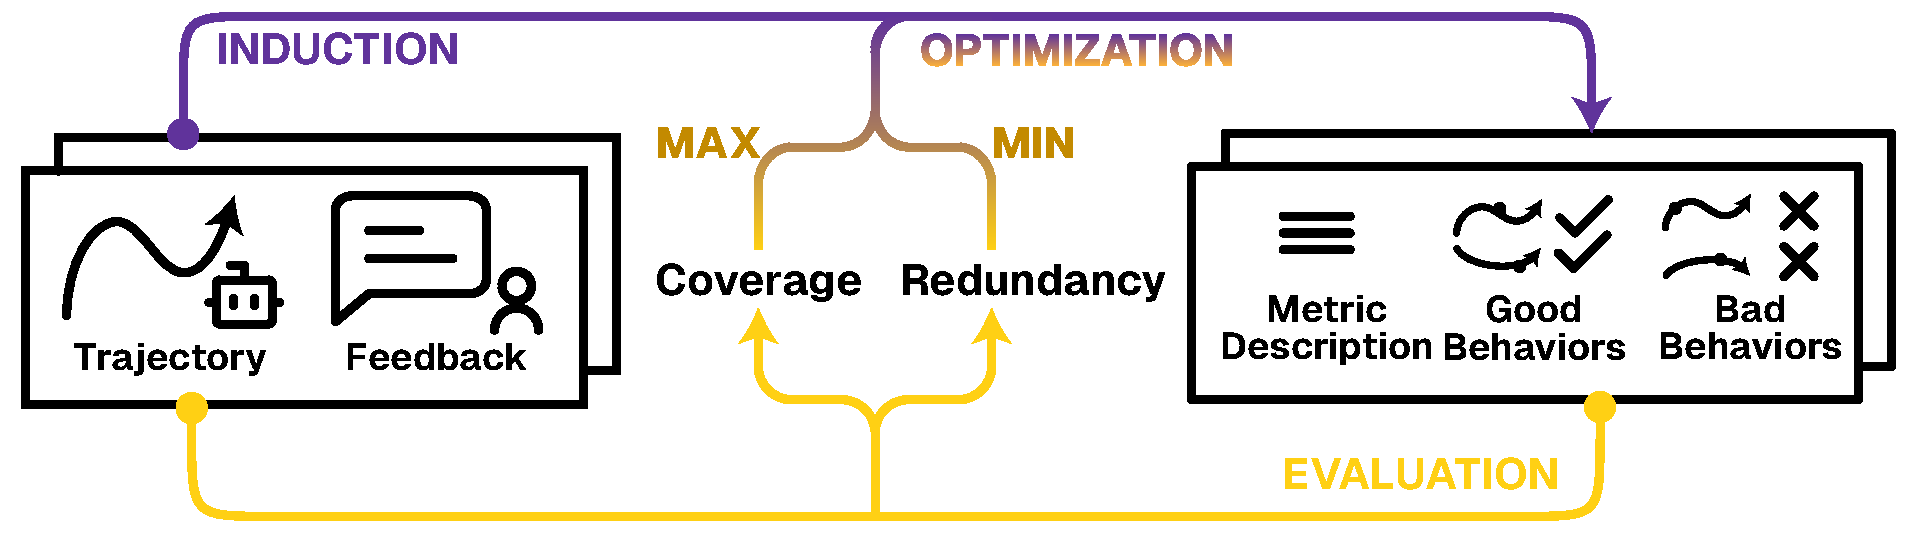
\includegraphics[width=0.8\linewidth]{figs/autolibra_optimization.pdf}
    \caption{Metric optimization: optimizing the induction process through maximizing the coverage while minimizing redundancy of the metrics, calculated via the evaluation process.}
    \label{fig:autolibra_optimization}
\end{figure}


As illustrated in Fig. \ref{fig:autolibra_optimization}, we tune the metric induction process to maximize coverage and minimize redundancy.
Among the two, we prioritize coverage of the metrics to provide a comprehensive evaluation of the agent behavior,
while minimizing overlap within the metrics to avoid redundancy.
To optimize for this objective, we generate 20 different metrics with $N$ ranging from 4 to 13,
and calculate the coverage and redundancy of the metrics in human feedback.
We then select metrics with a coverage of at least the highest coverage minus 1\%,
and the lowest redundancy.
This is performed iteratively, by resetting the range of $N$ to the number of metrics selected
previously $\pm$2, repeating until the coverage and redundancy
of the selected metrics converge, normally within 3 iterations.
While this optimization process is simple, experiments with various other optimization
strategies, including genetic algorithms and iterative clustering saw none of them
yield better results than the simple strategy.
\begin{wrapfigure}[24]{r}{0.6\textwidth}

    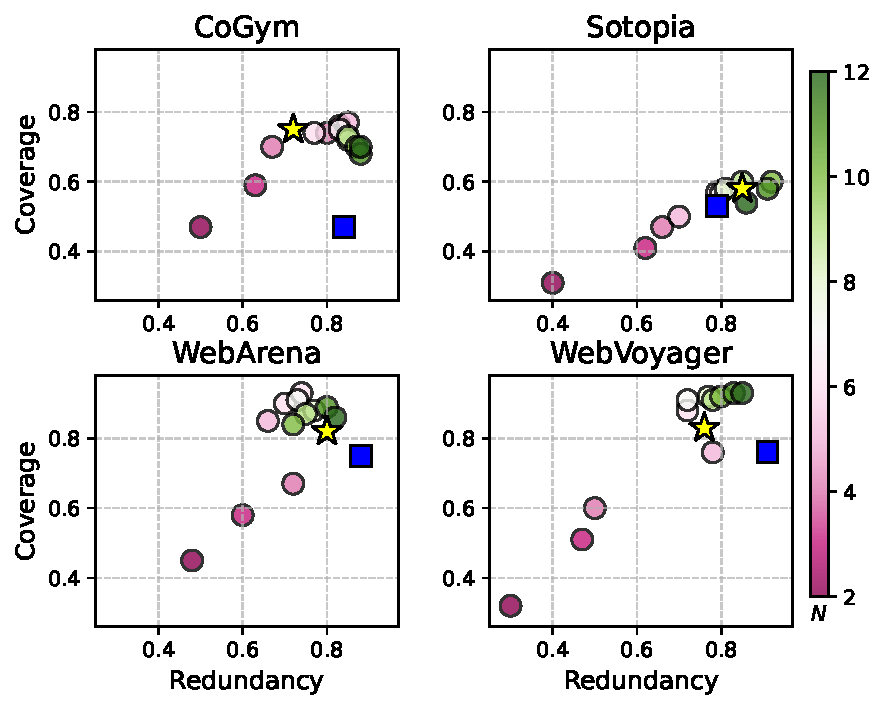
\includegraphics[width=0.6\textwidth]{figs/four_datasets_grid.pdf}
    \vspace{-15pt}  
    \caption{Coverage and redundancy of AutoLibra metrics on four agentic datasets. Circles indicate coverage
    and redundancy for different induced metrics; stars indicate the the best metrics' coverage and redundancy on held-out human feedback; squares indicate metrics without good and bad behaviors as examples.}
    \label{fig:coverage-redundancy}
\end{wrapfigure}
Fig. \ref{fig:coverage-redundancy} shows the highest coverages of the metrics of size $N$, which converge around $N=6$ to $10$ depending on the datasets. The best coverage on Sotopia \citep{zhousotopia} is the lowest among all four datasets, $60\%$, likely due to the diversity of the tasks in the dataset, while coverage on WebArena \citep{zhouwebarena} and WebVoyager \citep{he2024webvoyager} are the highest, $88\%$. We also find that the coverage of the held-out trajectories is only slightly worse ($<5\%$) than the trajectories we use to induce the metrics, which is expected since we use the exact examples extracted from the latter. Lastly, we show that the good and bad behaviors are crucial in the metrics, dropping which resulting in up to $30\%$ coverage decrease (on CoGym \citep{shao2024collaborative}).



\subsection{Iterative Metric Induction}
\label{sec:iterative-induction}
When applying AutoLibra to agent optimization, we can iteratively induce new metrics, as agents develop new failure modes or new behaviors as they improve, which is useful for tracking agents' progress across different iterations.\footnote{Alternatively, a new set of metrics can be induced from scratch for each iteration -  in practice, we do not find that this results in any coverage loss, but we choose the former method for consistency} 
%For example, in the Baba-is-AI task \citep[\S\ref{sec:Baba-Is-AI}]{cloos2024babaaibreakrules}, the agent initially fails to recognize the win condition and acts randomly; after the agent improves with an in-context example in the prompt, the agent starts to follow existing win conditions, but fails to construct new win conditions. This was not mentioned in human feedback before the agent improvement, since the agent was too random to even reach the stage where constructing new win conditions is possible. Therefore, in the second iteration, a new metric \texttt{win-rule construction} should be induced to provide a new signal for further optimizing the agent.

%\diyi{did we do this, or is the below only a comment?}}

To do this, we modify the behavior clustering step, by providing the LLM with the existing metrics
and their definitions, and ask the LLM not to change the definitions of the existing metrics, 
to only add new behaviors to the existing metrics, and add new metrics if necessary.
We apply the same optimization strategy as in the metric optimization step
ensure the newly induced metrics cover emerging behaviors and do not overlap with existing metrics.

\subsection{Validating AutoLibra-Human Alignment}

To measure the alignment of AutoLibra with human judgment,
we validate the feedback grounding, LLM-as-a-Judge, and Meta Evaluation steps through an additional human annotation stage (with exception of the behavior clustering step, as it is prohibitively time-intensive for human annotators to
process and cluster more than 400 aspects). The coverage and redundancy scores, in combination with the validation results of the other steps in the loop, thus serve as an indirect validation for the behavior clustering step.
Table \ref{tab:validation} shows the agreement rate of human annotators in AutoLibra steps. 
It should be noted that these tasks are vastly different; e.g., grounding for WebVoyager \citep{he2024webvoyager} is quite hard
due to the length and wide action space of the trajectory, and LLM-as-a-Judge for Sotopia \citep{zhousotopia} is
difficult due to the complexity of the evaluation of social interactions. 

\begin{table}[!t]
    \centering
    \small
    \begin{tabular}{cccccc|c}
        \toprule
        Steps & CoGym & Sotopia & WebArena & WebVoyager & Baba-is-AI & Average  \\
        \midrule
        Grounding & 0.95 & 0.95 & 0.98 & 0.93 & 0.93 & 0.95 \\
        LLM-as-a-Judge & 0.90 & 0.85 & 0.95 & 1.00 & 0.90 & 0.92 \\
        Meta-Evaluation & 0.98 & 0.90 & 0.85 & 0.83 & 0.95 &  0.90 \\
        \bottomrule
    \end{tabular}
    \caption{
        The ratio of instances marked as fully correct in human validation. For each step and
        each task, we randomly sample 40 instances and ask human annotators to label them as completely correct
        or not. Although the agreement scores vary across tasks and steps, the average agreement for each
        step and dataset is above 0.9. 
}
    \label{tab:validation}
\end{table}

%\diyi{S2 would benefit from a bit reorg. if you want, you can put 2.1, 2.2, 2.3 into one new subsection "Introducing AutoLibra (Pipeline)", and then use them as subsubsections; i would merge 2.4 and 2.5 as a second new subsection "Optimizing AutoLibra" and put the original 2.4 and 2.5 as subsubsections within it, to create more logic structures. i would move 2.6 to S3 as how you set up the initialization for using autolibra, etc.}